\section{MOS Operationsverstärker}
'Operationsverstärker' ist ein \textbf{Sammelbegriff} für Differenzverstärker mit sehr grosser Verstärkung.

\smallskip

Der \textbf{ideale} Operationsverstärker erfüllt zwei Bedingungen:
\begin{itemize}
    \item Es fliesst kein Strom in die Eingänge
    \item Die Spannungsdifferenz zwischen den Eingängen ist null
\end{itemize}

\medskip

Man unterscheidet dabei zwischen \textbf{zwei Arten} von Operationsverstärkern:
\begin{description}
    \item[OTA:] Der Transimpedanz-Operationsverstärker hat eine Spannung am Eingang und liefert am Ausgang einen Strom
    \item[OpAmp:] Der OpAmp verstärkt die Eingangsspannung zu einer Ausgangsspannung 
\end{description}

\begin{ctabular}{|c|c||c|c|}
    \hline
    \multicolumn{2}{|c||}{\textbf{OTA}}                 & \multicolumn{2}{c|}{\textbf{OpAmp}}           \\
    \hline
    $Z_{\rm in} \to \infty$ & $Z_{\rm out} \to \infty$  & $Z_{\rm in} \to \infty$ & $Z_{\rm out} \to 0$ \\
    \hline
\end{ctabular}

\vspace{-0.2cm}


\subsection{Struktur}

\begin{center}
    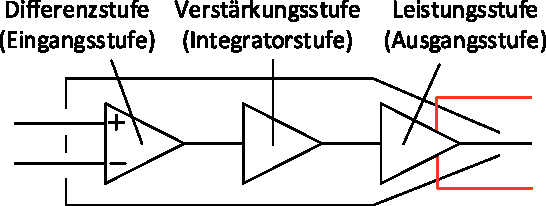
\includegraphics[width=0.65\columnwidth]{images/09_OpAmp_struktur.pdf}
\end{center}

\begin{outline}
    \1 \textbf{Differenzstufe}
        \2 Bildet die Differenz zwischen $V+$ und $V-$ und verstärkt diese
    \1 \textbf{Verstärkerstufe}
        \2 Erhöht die Verstärkung und bestimmt meist die Bandbreite
    \1 \textbf{Leistungsstufe}
        \2 Wandelt die hohe Impedanz in eine kleine Ausgangsimpedanz
            \textrightarrow\ \textbf{fehlt beim OTA}
\end{outline}


% \subsubsection{Differenzstufe}
% Bildet die Differenz zwischen $V+$ und $V-$ und verstärkt Differenzstufe

% \subsubsection{Verstärkerstufe}
% Erhöht die Verstärkung und bestimmt meist die Bandbreite.

% \subsubsection{Leistungsstufe}
% Wandelt die hohe Impedanz in eine kleine Ausgangsimpedanz.
% Diese Stufe fehlt beim OTA.


\subsection{Differenzstufe -- Grosssignalanalyse}

\subsubsection{Strong Inversion}

\begin{minipage}[t]{0.48\columnwidth}
    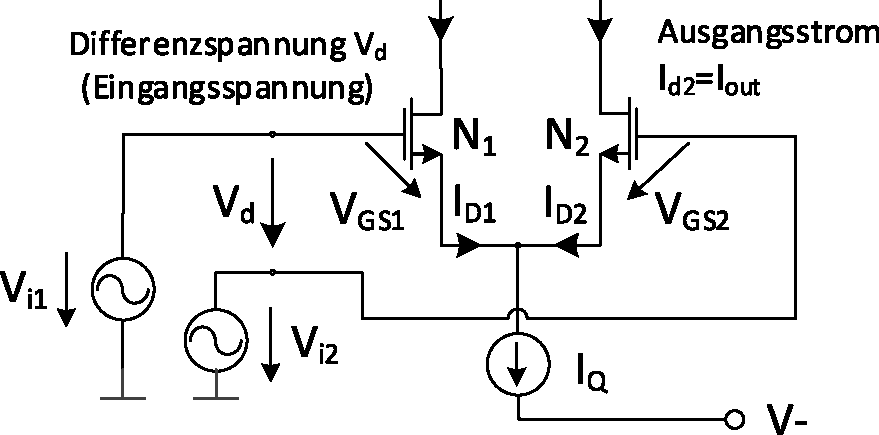
\includegraphics[width=\columnwidth, align=t]{images/09_differenzstufe_grosssignalanalyse.pdf}
\end{minipage}
\hfill
\begin{minipage}[t]{0.48\columnwidth}
    \begin{align*}
        \text{Sättigung:} \quad     I_\text{D}  &= \frac{\mu C_\text{ox}}{2} \frac{W}{L} (V_\text{GS} - V_\text{T})^2    \\
        \text{Konten:} \quad        I_\text{Q}  &= I_\text{D1} + I_\text{D2} 
    \end{align*}
\end{minipage}

\[
    \frac{I_\text{D}}{I_\text{Q}} = f(V_{\rm d}) = f(V_{i1} - V_{i2}) = \frac{1}{2} + \frac{1}{2} \sqrt{\frac{\left(\mu C_\text{ox} \frac{W}{L}\right) \cdot V_\text{d}^2}{I_\text{Q}} - \frac{\left(\mu C_\text{ox} \frac{W}{L}\right)^2 \cdot V_\text{d}^4}{4 I_\text{Q}}}
\]


%TODO: [Flurin] Kennlinie aus V10S9
%CHECK: [Simi] @Flurin: There it is... Eventuell ist es aber besser, die 3 Bereiche formelmässig darzustellen und die Grafik wegzulassen...?
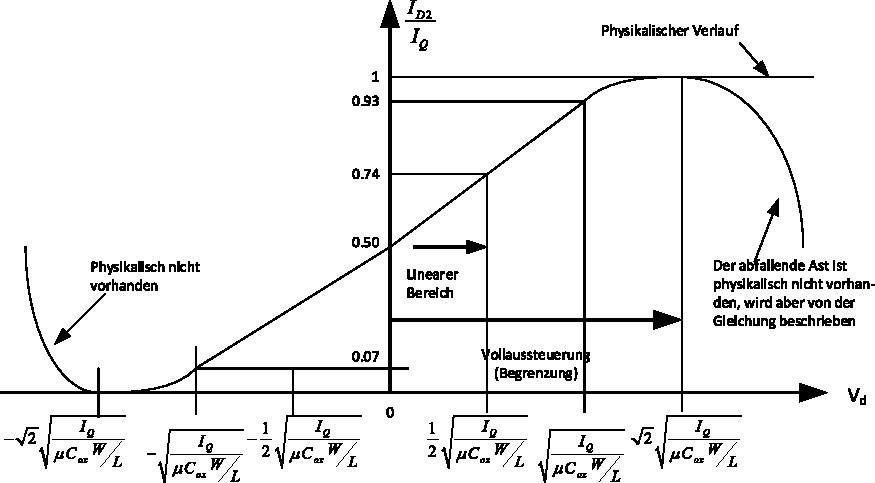
\includegraphics[width=\columnwidth, align=t]{images/09_differenzstufe_grosssignalanalyse_strong_inv.pdf}


\subsubsection{Weak Inversion}

\vspace{-0.2cm}

\[
    \text{Weak Inversion, Sättigung:} \qquad I_\text{D} = \frac{W}{L} I_\text{M}' e^\frac{V_\text{GS}-V_\text{M}}{n_\text{M} V_\text{temp}}
\]

\vspace{-0.2cm}

\[
    \frac{I_\text{D}}{I_\text{Q}} = f(V_{\rm d}) = f(V_{i1} - V_{i2}) = \frac{1}{2} \left(1 + \tanh \left( \frac{V_\text{d}}{2 n_\text{M} V_\text{temp}} \right) \right)
     \overset{V_d \text{ klein}}{\approx} \frac{1}{2} \left(1+\frac{V_\text{d}}{2 n_\text{M} V_\text{temp}}\right)
\]


\subsubsection{Conclusion Grosssignalanalyse}

Die \textbf{Verstärkung} ist im grossen und ganzen \textbf{unabhängig} von der Eingangsspannung und so \textbf{vom Arbeitspunkt}, der durch die Eingangsspannungen gegeben ist.

\smallskip

Der Ausgangsstrom hängt nur von der \textbf{Differenz der Eingangsspannungen} ab, was zu Linearität in einem grossen Bereich führt.


\subsection{Differenzstufe -- Kleinsignalanalyse}

\subsubsection{Transkonduktanz $\bm{g_{\rm md}}$}

\begin{minipage}[t]{0.48\columnwidth}
    \paragraph{Widerstandslast}

    \[
        g_{\rm md} = \frac{i_{\rm out}}{v_{\rm d}} = - \frac{g_m}{2}
    \]
\end{minipage}
\hfill
\begin{minipage}[t]{0.48\columnwidth}
    \paragraph{Stromspiegellast}

    \[
        g_{\rm md} = \frac{i_{\rm out}}{v_{\rm d}} = - g_m
    \]
\end{minipage}


% TODO: [Flurin] Evtl. Schema und Ersatzschaltbild aus V10S11
%CHECK: [Simi] @Flurin There it is aber ich würde es weglassen... Habe im Bild weiter oben den 'Ort' eingefügt, wo die Last hin muss
% -> wenn du die Bilder verwenden willst, müsste man wahrscheinlich etwas umformatieren und herumschieben...

% \paragraph{Widerstandslast}

% \begin{minipage}[t]{0.45\columnwidth}
%     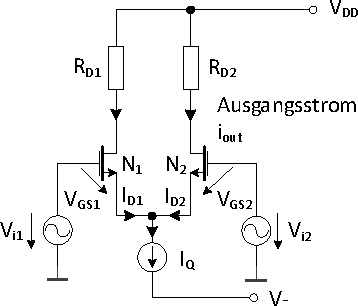
\includegraphics[width=\columnwidth, align=t]{images/09_differenzstufe_widerstandslast_schaltung.pdf}
% \end{minipage}
% \hfill
% \begin{minipage}[t]{0.45\columnwidth}
% 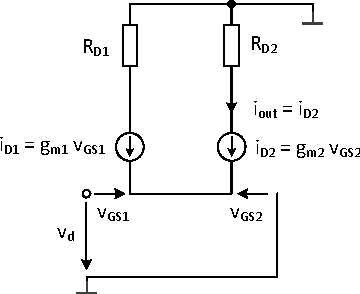
\includegraphics[width=\columnwidth, align=t]{images/09_differenzstufe_widerstandslast_kleinsignal.pdf}
% \end{minipage}


% \paragraph{Stromspiegellast}

% TODO: [Flurin] Evtl. Schema und Ersatzschaltbild aus V10S11
%CHECK: [Simi] @Flurin There it is aber ich würde es weglassen... Habe im Bild weiter oben den 'Ort' eingefügt, wo die Last hin muss
% -> wenn du die Bilder verwenden willst, müsste man wahrscheinlich etwas umformatieren und herumschieben...

% \begin{minipage}[t]{0.45\columnwidth}
%     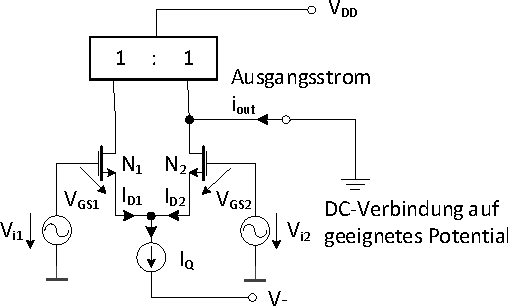
\includegraphics[width=\columnwidth, align=t]{images/09_differenzstufe_stromspiegellast_schaltung.pdf}
% \end{minipage}
% \hfill
% \begin{minipage}[t]{0.45\columnwidth}
%     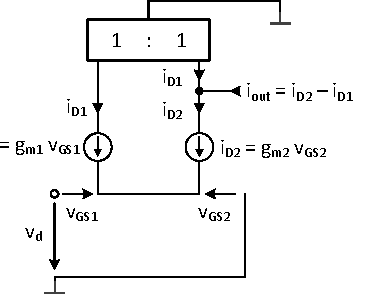
\includegraphics[width=\columnwidth, align=t]{images/09_differenzstufe_stromspiegellast_kleinsignal.pdf}
% \end{minipage}



\subsubsection{Verstärkung}

Generell berechnet sich die Verstärkung der Differenzstufe $a_{\rm Diff}$ als 

\[
    a_{\rm Diff} = \frac{v_{\rm out}}{v_{\rm in}} = g_{\rm md} \cdot r_{\rm Last\_tot}
\]

\begin{outline}
    \1 Abhängig von der Last muss $g_{\rm md}$ entsprechend eingesetzt werden
    \1 $r_{\rm Last\_tot}$ entspricht der gesamten Last am Ausgangsknoten
\end{outline}


\paragraph{Widerstandslast}

\begin{minipage}[t]{0.45\columnwidth}
    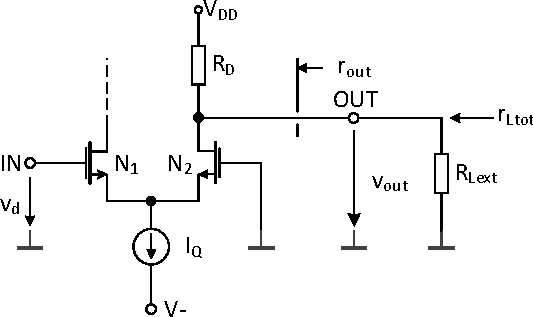
\includegraphics[width=\columnwidth, align=t]{images/09_differenzstufe_kleinsignal_verstaerkung_widerstand.pdf}
\end{minipage}
\hfill
\begin{minipage}[t]{0.5\columnwidth}
    \[
        r_{\rm Last\_tot} = \left( R_D \parallel r_{\rm DS} \parallel R_{\rm Lext} \right) \approx \left( R_D \parallel R_{\rm Lext} \right) 
    \]

    \[
        a_{\rm Diff} \approx - \frac{g_m (R_D \parallel R_{\rm Lext})}{2}
    \]
\end{minipage}



\paragraph{Stromspiegellast}

\begin{minipage}[t]{0.45\columnwidth}
    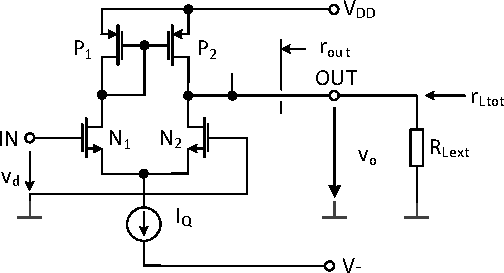
\includegraphics[width=\columnwidth, align=t]{images/09_differenzstufe_kleinsignal_verstaerkung_stromspiegel.pdf}
\end{minipage}
\hfill
\begin{minipage}[t]{0.5\columnwidth}
    \[
        r_{\rm Last\_tot} =  \left( r_{\rm DS\_N2} \parallel r_{\rm DS\_P2} \parallel R_{\rm Lext} \right)
    \]

    \vspace{-0.2cm}

    \[
        a_{\rm Diff} \approx - g_m \left(\frac{1}{g_{\rm o, N2}} \Biggm\Vert \frac{1}{g_{\rm o, N2}} \Biggm\Vert R_{\rm Lext}\right)
    \]
\end{minipage}


% \[
%     a \approx g_m \left(\frac{1}{g_{0, N2}} \Biggm\Vert \frac{1}{g_{0, N2}} \Biggm\Vert R_{L\text{, ext}}\right)
% \]


\paragraph{Stromquellenlast}    % NOTE: [Simi] Hat er nicht besprochen, daher verzichte ich hier auf das Schema

\vspace{-0.2cm}



\[
    r_{\rm Last\_tot} =  \left( r_{\rm QL} \parallel r_{\rm DS2} \parallel R_{\rm Lext} \right) \qquad \qquad
    a_{\rm Diff} \approx \frac{ \left( R_{\rm Lext} \parallel r_{\rm DS2} \parallel r_{\rm QL} \right) }{2}
\]



\subsubsection{Grenzwertbetrachtungen der Spannungsverstärkung}

Für folgende Grenzwertbetrachtungen der Spannungsverstärkung gilt: $R_{\rm Lext} = \infty$

\resizebox{\columnwidth}{!}{
    \begin{tabular}{|l|l|l|}
        \hline
        \textbf{Betriebsbereich}    & \textbf{Grenzwert der Spannungsverstärkung}                                                                                                       & \textbf{Grössere Verstärkung bei}                                         \\
        \hline
        Strong Inversion            & $\displaystyle \abs{a_{\text{max}}} = 2 V_e \sqrt{\frac{\mu C_\text{ox} \frac{W}{L}}{I_Q}} \approx 2 a_E \sqrt{\frac{\mu C_\text{ox} L W}{I_Q}}$  & Ruhestrom $\downarrow$, Fläche $\uparrow$, (Early-Spannung $\uparrow$)    \\
        \hline
        Weak Inversion              & $\abs{a_{\text{max}}} = \frac{V_E}{n_M V_\text{temp}} \approx \frac{a_E L}{n_M V_\text{temp}}$                                                    & (Early-Spannung $\uparrow$)                                               \\
        \hline
    \end{tabular}
}

\medskip

Diese Formeln sollten \textbf{nicht zur Verstärkungsberechnung verwendet werden} -- sie dienen lediglich zur Darstellung der Bezüge verschiedener Parameter.
% TODO: [Flurin] Evtl mehr Formeln / Bedingungen aus V10S14?
% [Simi] @Flurin: Ich würde nicht... Wir dürfen damit ja sowieso nicht rechnen....


